\documentclass{article}
\usepackage[utf8]{inputenc}
\usepackage[german]{babel}
\usepackage[T1]{fontenc}

\usepackage{xcolor}
\usepackage{listings}
\usepackage{graphicx}
\usepackage{hyperref}
\usepackage{grffile}

\usepackage{nasm/lang}
\usepackage{nasm/style}
\usepackage{c/style}

\usepackage{xparse}

\NewDocumentCommand{\codeword}{v}{
	\texttt{\textcolor{blue}{#1}}
}

\title{ERA-Projekt 1 - Dokumentation}
\author{Till Müller}
\begin{document}

\maketitle

\tableofcontents

\newpage

\section{Nutzerdokumentation}

\subsection{Grundprogramm}

	Das Grundprogramm wird über die Kommandozeile aufgerufen und
	bekommt optional eine Zahl z als Argument übergeben, und gibt
	den Arkussinus dieser Zahl aus.

	\vspace{0.3cm}

	Hierbei ist der \codeword{Routine output} die Ausgabe des eigens
	geschriebenen Arcsinus \codeword{doit()}, und der \codeword{Library output} die Ausgabe der Funktion \codeword{asin()} aus
	der C-Standardbibliothek.  Wurden keine Argumente auf der
	Kommandozeile übergeben, ist z automatisch auf 1 gesetzt.

	\vspace{0.3cm}

	Die Funktion \codeword{doit(f)} gibt hierbei den Arcsinus
	des Floating-Point Wertes f zurück, falls \(-1\leq f \leq 1\),
	andernfalls wird 2 zurückgegeben.

	\subsection{Kompilieren und Ausführen des Programms}
	Um das Programm kompilieren und somit ausführen zu können,
	werden folgende Bibliotheken und Programme benötigt:

	\begin{tabular}{l | p{15mm} | p{60mm}}
		Programm & Getestete Version & Funktionalität\\
		\hline
		svn (Subversion) & 1.9.3 & Ermöglicht einen Download der aktuellen Quelldateien\\
		nasm (Netwide Assembler) & 2.11.08 & Kompiliert die in NASM-Syntax geschriebene Routine\\
		gcc-Toolchain & 5.4.0 & Kompiliert und linkt das Rahmenprogramm und die Tests zur Routine\\
		make & 4.1 & Wird verwendet um den Prozess des Kompilierens zu spezifizieren und auszuführen\\
	\end{tabular}

	\emph{Hinweis: Da die Routine und somit auch Rahmenprogramm und Tests für 32-bit
	Systeme geschrieben und getestet wurden, kann es Probleme auf 64-bit Systemen geben.
	Diese lassen sich meistens durch die Installation von 32-bit-Versionen der
	Bibliotheken und Programme (sofern verfügbar) beheben.}

	\begin{figure}[hb]
		\centering
		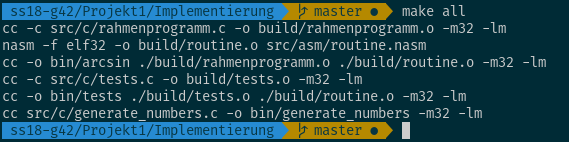
\includegraphics[width=0.7\linewidth]{images/makeshot}
		\caption{Erfolgreiches \emph{make}}
		\label{fig:screenshotmake}
	\end{figure}

	Bei gegebenen Voraussetzungen erfolgt die Kompilierung des
	Programmes durch den einfachen Befehl \codeword{make}.
	Dadurch werden, wie in Abb. \ref{fig:screenshotmake} zu sehen,
	die korrespondierende Quelldateien in der
	benötigten Reihenfolge kompiliert und verlinkt.
	Um die erstellten Dateien wieder zu löschen, wird ein \codeword{make clean}
	ausgeführt, welches das \emph{build-} und \emph{bin} Verzeichnis leert und löscht.

	Nach einer erfolgreichen Kompilierung liegt das Rahmenprogramm,
	welches die Assembler-Routine aufruft,
	 in dem Ordner \emph{bin/arcsin}.
	 Die Ausführung des Rahmenprogrammes, erfolgt durch den Befehl
	\codeword{./bin/arcsin [number]}, wobei \codeword{[number]} optional ist,
	wenn gegeben aber eine Zahl zwischen -1.0 und 1.0 sein sollte.
	\begin{figure}[hb]
		\centering
		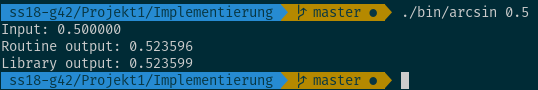
\includegraphics[width=0.7\linewidth]{images/arcsucc}
		\caption{Erfolgreiches \emph{./bin/arcsin 0.5}}
		\label{fig:arcsucc}
	\end{figure}
	\begin{figure}[htb]
		\centering
		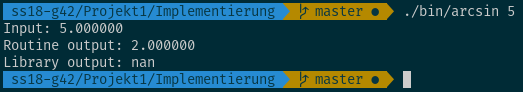
\includegraphics[width=0.7\linewidth]{images/arcfail}
		\caption{Fehlschlag bei: \emph{./bin/arcsin 5}}
		\label{fig:arcfail}
	\end{figure}

	Wenn kein Wert gegeben wird, wird der Arkussinus für den Wert 1.0 ausgeben,
	sonst der gegebene Wert berechnet, ggf. interpoliert und dann
	zurückgegeben, wie in Abb. \ref{fig:arcsucc} zu sehen.
	Für Werte, die außerhalb dieses Bereiches liegen, gibt die implementierte
	Routine immer den Wert 2 (siehe \ref{fig:arcfail}) aus,
	der außerhalb des Wertebereiches des Arkussinus liegt.

		\begin{figure}[hb]
			\centering
			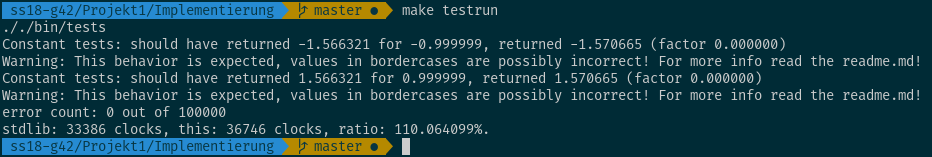
\includegraphics[width=1.0\linewidth]{images/testrun}
			\caption{\emph{make testrun}}
			\label{fig:testrun}
		\end{figure}

		Die Ergebnisse aus der Routine, werden mit denen der C-Bibliotheksfunktion verglichen
		und Resultate ausgegeben (siehe Abb. \ref{fig:testrun}.

		\subsection{Tests hinzufügen}
		\begin{enumerate}
			\item Zum Hinzufügen von Tests die Datei \emph{src/c/tests.c} bearbeiten: \begin{itemize}
				\item In das Array \codeword{test_value} in Zeile 11 Wertepaare hinzufügen. \begin{itemize}
					\item In der Form \codeword{{[Eingabewert], [erwarteter Ausgabewert]}}
					\item Beispielsweise  \codeword{{[0], [0]}}
				\end{itemize}
				\item \textbf{Alternativ:} Für komplexere Tests der \codeword{main}-Methode eine Routine hinzufügen
			\end{itemize}
			\item \codeword{make clean}, \codeword{make} und \codeword{make testrun} aufrufen, um alle Tests auszuführen.
		\end{enumerate}

	\subsection{Genauigkeit der Tests}

	Ein Vergleich zweier Ergebnisse ist dann erfolgreich, wenn das
	500-fache beider Zahlen, abgerundet, die gleiche Zahl ist.

	\vspace{0.3cm}

	Hierbei werden zuerst Konstanten an den Rändern des
	Wertebereiches (-1.000001, -1, -0.999999 und die positiven
	Äquivalente) und Zahlen nahe an der Null (-0.000001, 0,
	0.000001) auf ihre Korrektheit getestet. Die Ungenauigkeiten
	treten hierbei aufgrund starker Veränderungen der Funktionswerte
	an den Randbereichen auf, da dort der Arkussinus besonders
	schnell ansteigt und damit die Interpolation immer ungenauer
	wird, je weiter der übergeben Wert sich der 1 beziehungsweise
	der -1 annähert. Aus diesem Grund wird das Funktionsresultat
	über zwei Tabellen berechnet, eine für Argumente kleiner
	als 0.9 und eine für Argumente größer als 0.9.

	\vspace{0.3cm}

	Daraufhin wird eine fix festgelegte Anzahl (default 100000)
	von zufälligen Zahlen innerhalb des zulässigen Wertebereiches
	\(-1\leq x \leq 1\) in \codeword{doit()} und \codeword{asin()}
	eingesetzt und die Ergebnisse werden verglichen. Währenddessen
	werden die Laufzeiten der beiden Funktionen in unabhängigen
	Variablen aufsummiert und am Ende miteinander verglichen.
	Clocks sind hierbei die Takte des Prozessors. Normalerweise
	ist diese Implementierung 30\% bis 40\% langsamer als die
	Implementierung in der C-Standardbibliothek.

\newpage

\section{Entwicklerdokumentation}

\subsection{rahmenprogramm.c}

	Diese Datei enthält das Hauptprogramm, das das Argument auf der
	Kommandozeile entgegennimmt und daraufhin die Ergebnisse der
	Berechnungen ausgibt. Die Zeile

\vspace{0.3cm}


\begin{lstlisting}[language=c,style=c]
extern float doit(float);
\end{lstlisting}

\vspace{0.3cm}

	definiert die Funktion \codeword{doit()} als eine Funktion,
	die durch eine andere Objektdatei eingebunden wird.

\subsection{routine.asm}

	Diese Datei bildet das Herzstück des Programmes: sie implementiert
	die Funktion \codeword{doit(float x)}, welche für den Wert x eine 
	möglichst genaue Annäherung \codeword{float y} 
	$y = sin^{-1}(x)$ zurückgibt.

	\vspace{0.3cm}

	Sie ist in mehrere Abschnitte unterteilt. Zuerst erfolgt die
	Initialisierung des Programmes, in der der Wertebereich der
	Eingabe überprüft wird. Daraufhin folgt die Berechnung der
	Adresse des Eingabewerts in der Tabelle. Danach prüft der Code,
	ob eine Interpolation notwendig ist, und führt diese, falls nötig, durch.
	Andernfalls wird der Wert direkt aus der entsprechenden
	Tabelle geladen und zurückgegeben.
	Schlussendlich wird, falls notwendig, das Vorzeichen des
	Rückgabewertes gesetzt und die auf dem Stack gespeicherten Werte
	zurück in ihre Register geschrieben.

\subsubsection{Bereitstellung des verwendeten Speichers und Konstanten}

	Zunächst werden in der Sektion \codeword{.bss} folgende Speicher-
	bereiche reserviert:

\vspace{0.5cm}

\lstset{language=nasm, style=nasm}

\begin{lstlisting}
section .bss
index_1:        resd 1
index_2:        resd 1
res:            resd 1
cw:             resw 1
flag:           resd 1
\end{lstlisting}

\vspace{0.5cm}

	Hierbei haben die Speicherbereiche folgende Verwendungszwecke:

	\begin{itemize}
	\item flag: Das untersten Bit dieses Speicherbereiches ist gesetzt,
	wenn die Eingabe \(f\) negativ war. Das vorunterste Bit ist dann
	gesetzt, wenn \(abs(f)\geq 0.9\) ist.
	\item index\_1: Wird benutzt, um die nach unten abgerundete
	Adresse bei der Interpolation zu speichern. Dieser Speicherbereich
	wird auch dann für den Wert benutzt, wenn keine Interpolation
	notwendig ist.
	\item index\_2: Wird benutzt, um die nach oben abgerundete
	Adresse bei der Interpolation zu speichern.
	\item res: Wird benutzt, um bei der Interpolation den Eingabewert
	zwischenzuspeichern.
	\item cw: Wird bei der Interpolation benutzt, um das Kontrollwort der
	FPU zwischenzuspeichern, bevor die Werte in der FPU gerundet werden.
	\end{itemize}

	Daraufhin werden die folgenden Konstanten definiert:

\vspace{0.5cm}

\begin{lstlisting}
two:            dd 2.0
ten:            dd 10.0
pnine:          dd 0.9
size_main:      dd 1000
size_high:      dd 1000
\end{lstlisting}

\vspace{0.5cm}

	sowie die beiden Tabellen \codeword{table_main} und \codeword{table_high}.
	Die ersten 3 Konstanten sind selbsterklärend, die letzten beiden geben
	die Größen der beiden Lookup-Tables mit den Werten des Arkussinus an.

\subsubsection{Initialisierung der Funktion und Prüfen des Eingabewertes}

	Anfangs werden die Werte aus den verwendeten Registern auf
	den Stack gepusht, der Inhalt von \codeword{flag} zurückgesetzt 
	und die FPU auf einen Startzustand zurückgesetzt, 
	um undefiniertes Verhalten bei wiederholten Routinenaufrufen zu vermeiden.
	Das Funktionsargument steht zu Beginn an der Adresse \codeword{esp+4}.
	Da sich der Stackpointer bekannterweise bei weiteren Stack-Verwendungen verändert,
	wird zuerst der Basepointer gesichert, anschließend auf den Wert des Stackpointers gesetzt,
	somit ändert sich die Adresse des Arguments für den Ablauf der Routine zu \codeword{ebp+8}.
	Dieser Wert dann in das FPU-Register geladen und steht in \codeword{st0}.

\vspace{0.5cm}

\begin{lstlisting}
push ebp
mov ebp, esp
push eax
push ebx ; ebx: table address

; reset flag
xor eax, eax
mov [flag], eax

finit ; initialize fpu
fld dword [ebp+8] ; st0 = val
\end{lstlisting}

\vspace{0.5cm}

	Daraufhin prüft die Funktion mittels \codeword{fcomp}, ob das 
	Funktionsargument innerhalb
	von \([-1;1]\) liegt. Liegt es nicht innerhalb dieses Intervalls, wird
	zu \codeword{out_of_range} gesprungen, das \emph{2} als ungültigen Wert
	 in die FPU lädt und zur \codeword{end}Routine springt.

\vspace{0.5cm}

\begin{lstlisting}
; check for edge-cases
fld1 ; load 1
fchs ; negate
fcomp ; compare st0 and st1
fstsw ax ; store status register
and eax, 0100011100000000B ; filter out status bits
cmp eax, 0000000000000000B ; check if st0 > st1 (val < -1.0)
je out_of_range

fld1; load 1
fcomp ; compare st0 and st1
fstsw ax ; store status register
and eax, 0100011100000000B ; filter out status bits
cmp eax, 0000000100000000B ; check if st0 < st1 (val > 1.0)
je out_of_range
\end{lstlisting}

\vspace{0.5cm}

	Um später das Ergebnis mit korrektem Vorzeichen anzugeben,
	wird jetzt das Vorzeichen des Funktionsarguments im untersten
	Bit gespeichert und ab dann der absolute Wert des Arguments
	weiterverwendet.
	Die Vorzeichenbestimmung erfolgt wie oben mittels \codeword{fcomp},
	wodurch der Eingabewert mit 0 (\codeword{fldz} lädt 0 in das oberste Register),
	verglichen wird.

\vspace{0.5cm}

\begin{lstlisting}
fldz
fcomp
fstsw ax;
and eax, 0100011100000000B ; filter out status bits
cmp eax, 0000000000000000B ; check if st0 > st1 (val < 0.0)
je negative
jmp table_check
negative:
mov eax, 01b
mov [flag], eax
xor eax, eax
\end{lstlisting}

\subsubsection{Wählen der Lookup-Tabelle}

	Der nächste Schritt im Programm besteht im 
	Wählen der passenden Lookup-Tabelle 
	für die entsprechende Eingabe. Hierbei wird
	unterschieden, ob das Funktionsargument größer oder kleiner
	als 0.9 ist. Im ersten Fall wird die Adresse im Abschnitt
	\codeword{set_high} in der Tabelle \codeword{table_high} bestimmt,
	im zweiten Fall im Abschnitt \codeword{main_high} in der Tabelle
	\codeword{table_main}. Die Adresse der verwendeten Tabelle wird
	in \codeword{ebx} abgelegt.
	

\vspace{0.5cm}

\begin{lstlisting}
fld dword [pnine]
fcomp
fstsw ax;
and eax, 0100011100000000B ; filter out status bits
cmp eax, 0000000100000000B ; check if st0 < st1 (val > 0.9)
je set_high
jmp set_main
\end{lstlisting}

\vspace{0.5cm}

	In \codeword{set_high} wird zuerst das vorunterste Bit in
	\codeword{flag} gesetzt, das indiziert, dass die Tabelle
	\codeword{table_high} verwendet wurde. Die Adresse von
	\codeword{table_high} wird in \codeword{ebx} gelegt.
	Da diese Tabelle mit einem Wertebereich von 0.9 - 1.0
	zehn mal so genau wie \codeword{table_main} ist, muss zusätzlich
	zu der Skalierung zur \codeword{size_high}, eine 10-fache Skalierung geschehen.
	Die Gesamtskalierung ist für diese Tabelle also wie folgt definiert:
	\[\textrm{scale} = size\_high \cdot 10\]
	Außerdem beinhaltet die Tabelle nur Werte für 0.9 - 1.0, 
	die erste Zahl für den Wert $sin^{-1}(0.9)$, liegt an Index 0;
	Somit muss zusätzlich ein Offset abgezogen werden, hier berechnet es sich durch:
	\[\textrm{offset} = 10 * size\_high\]
	Das fasst sich zusammen zu:
	\[input = (input \cdot size\_high \cdot 10)-(10 \cdot size\_high)\]
	Daraufhin wird zu
	\codeword{inter_check} gesprungen:

\vspace{0.5cm}

\begin{lstlisting}
mov ebx, table_high
mov eax, [flag]
or eax, 10b ; set table statusbit
mov [flag], eax

fimul dword [size_high]
fld dword [ten]
fmulp

fild dword [size_high]
fld dword [ten]
fmulp
fisub dword [size_high]
fsubp st1, st0 ; subtract from input

jmp inter_check
\end{lstlisting}
\newpage %TODO: Necessary?
\vspace{0.5cm}

	\codeword{set_main} ist deutlich weniger komplex. Hier
	wird die Skalierung $input = input*size\_main$ ausgeführt und
	\codeword{table_main} in \codeword{ebx} gespeichert:

\vspace{0.5cm}

\begin{lstlisting}
mov ebx, table_main
fimul dword [size_main]
\end{lstlisting}

\subsubsection{Interpolation}

	Als nächstes wird geprüft, ob eine Interpolation notwendig ist
	(also, ob der oberste Wert auf dem FPU-Stack gleich seinem
	gerundetem Äquivalent ist). Ist dies der Fall, wird zu
	\codeword{interpolate} gesprungen, ansonsten wird
	zu \codeword{equal} gesprungen:

\vspace{0.5cm}

\begin{lstlisting}
fld st0 ; duplicate stack top value
frndint
fcomp st0, st1
fstsw ax
and eax, 0100011100000000B ; filter out status bits
cmp eax, 0000000000000000B ; check if st0 > st1
je interpolate
cmp eax, 0000000100000000B ; check if st0 < st1
je interpolate
cmp eax, 0100000000000000B ; check if st0 = st1
je equal
jmp end
\end{lstlisting}

\vspace{0.5cm}

	Im Abschnitt \codeword{interpolate} werden zuerst der
	abgerundete Wert des ausgerechneten Tabellenindex in den
	Speicherbereich \codeword{index_1} und der aufgerundete Wert in
	den Speicherbereich \codeword{index_2} geschrieben. Dies wird
	dadurch erreicht, dass erst das Kontrollwort in der FPU gesetzt, dann die geschätzte Tabellenadresse ausgerechnet
	und schließlich die Instruktion \codeword{frndint} ausgeführt
	wird. Hierbei werden im Register eax erst die Flags gesetzt,
	dann wird es auf den Stack gepusht, von dem dann die FPU das
	Kontrollwort lädt.  Außerdem wird das oberste Element in der
	FPU in \codeword{res} gespeichert, dort liegt dann also die
	in \codeword{set_high} oder \codeword{set_main} ausgerechnete
	Adresse.

\vspace{0.5cm}

\begin{lstlisting}
; index_1 = floor(val)
fstcw [cw] ; save current control word
fwait

mov ax, [cw]
and ax, 0x0F3FF ; mask round-control bits
or  ax, 0x00700 ; set round-control bits to 01 (round down)
push eax ; push new control word to stack

fldcw [esp] ; load control word

fld st0 ; clone stack top
frndint ; round
fistp dword [index_1] ; store integer
pop eax

; index_2 = ceil(val)
and ax, 0x0F3FF ; mask round-control bits
or  ax, 0x00B00 ; set round-control bits to 10 (round up)
push eax ; push new control word to stack

fldcw [esp] ; load control word

fld st0 ; clone stack top
frndint ; round
fistp dword [index_2] ; store integer

fldcw [cw]
pop eax
fstp dword [res]
\end{lstlisting}

\vspace{0.5cm}

	Daraufhin wird mit der folgenden Formel

	\[y:=y_1+\frac{y_2-y_1}{x_2-x_1}*(x-x_1)\]

	interpoliert, das Ergebnis \(y\) wird dabei im FPU-Register \codeword{st0} abgelegt.
	Hierbei
	liegt \(x_1\) in \codeword{[index_1]}, \(x_2\) in \codeword{[index_2]},
	\(x\) in \codeword{res}, \(y_1\) in \codeword{ebx+[index_1]} und
	\(y_2\) in \codeword{ebx+[index_2]}:

\vspace{0.5cm}

\begin{lstlisting}
mov eax, [index_2]
fld dword [ebx+eax*4] ; load y2 into fpu
mov eax, [index_1]
fld dword [ebx+eax*4] ; load y1 into fpu

fsubp ; st0 =  y2 - y1

fild dword [index_2] ; st0 = x2
fisub dword [index_1] ; x2 - x1

fdivp ; st0 = (y2 - y1)/(x2 - x1)

fld dword [res] ; load val
fisub dword [index_1] ;(x - x1)

fmulp ;(st0 = st1 * (x-x1))

mov eax, [index_1]
fadd dword [ebx+eax*4] ; st0 + st1
\end{lstlisting}

\vspace{0.5cm}

	Besteht keine Notwendigkeit, das Ergebnis zu interpolieren,
	dann wird im Abschnitt \codeword{equal} der Inhalt der Tabelle
	mit dem Offset \codeword{st0} über \codeword{index_1} aus der
	Tabellenadresse im Register \codeword{ebx} auf den FPU-Stack
	geladen:

\vspace{0.5cm}

\begin{lstlisting}
fistp dword [index_1]
mov eax, [index_1]
fld dword [ebx+eax*4]
\end{lstlisting}

\vspace{0.5cm}

	Zuletzt wird im Abschnitt \codeword{end} das Ergebnis abhängig
	vom untersten Bit in \codeword{flag} negiert und die Register
	werden aus dem Stack wiederhergestellt, bevor die Funktion
	beendet wird.

\vspace{0.5cm}

\begin{lstlisting}
mov eax, [flag]
and eax, 1b ; filter out status flag
cmp eax, 1
jne exit
fchs ; negative: change sign
exit:
pop ebx
pop eax
pop ebp
ret
\end{lstlisting}

\subsection{tests.c}

	Das Programm tests wird verwendet, um \codeword{doit()}
	mit der Funktion aus der C-Standardbibliothek nach Korrektheit der Ergebnisse als auch nach der
	Performance zu vergleichen. Hierbei werden zuerst konstante Werte miteinander
	verglichen, insbesondere die folgenden (der Eingabewert steht
	auf der linken Seite, der erwartete Ausgabewert auf der rechten):

\vspace{0.5cm}

\lstinputlisting[language=c, style=c, firstline=11, lastline=22, firstnumber=11]{../Implementierung/src/c/tests.c}

\vspace{0.5cm}

	Das Programm definiert verschiedene Konstanten, nämlich

\vspace{0.5cm}

\lstinputlisting[language=c, style=c, firstline=7, lastline=9, firstnumber=7]{../Implementierung/src/c/tests.c}

\vspace{0.5cm}

	Diese Konstanten bedeuten:

	\begin{itemize}
	\item \codeword{FACTOR}: Der von \codeword{doit()} zurückgegebene Wert wird
	dann akzeptiert, wenn das FACTOR-fache dieses Wertes und das
	\codeword{FACTOR}-fache des erwarteten Wertes, abgerundet, die gleiche
	Zahl sind.
	\item \codeword{CONSTS}: Die Anzahl der Elemente in \codeword{test_value}.
	\item \codeword{RANDROUNDS}: Die Anzahl der Tests von von \codeword{doit()}
	mit zufälligen Werten.
	\end{itemize}

	Die Funktion within prüft, ob das Ergebnis von \codeword{doit()}
	ein akzeptable Ergebnis ist. Hierbei ist das Argument \codeword{res}
	das von \codeword{doit()} zurückgegebene Ergebnis, \codeword{fix}
	der Vergleichswert, und \codeword{margin} normalerweise \codeword{FACTOR}:

\vspace{0.5cm}

\lstinputlisting[language=c, style=c, firstline=37, lastline=40, firstnumber=37]{../Implementierung/src/c/tests.c}

\vspace{0.5cm}

	In der Funktion \codeword{main} wird zunächst getestet,
	ob die vorher definierten Konstanten die korrekten Ergebnisse
	haben. Hierbei wird einfach über \codeword{test_value} iteriert,
	der jeweils erste Wert an \codeword{doit()} übergeben und das
	Ergebnis dann mithilfe von \codeword{within} mit dem zweiten
	Wert aus \codeword{test_value} geprüft.

\vspace{0.5cm}

\lstinputlisting[language=c, style=c, firstline=50, lastline=57, firstnumber=50]{../Implementierung/src/c/tests.c}

\vspace{0.5cm}

	Daraufhin führt das Programm \codeword{RANDROUNDS} Tests mit zufälligen
	Werten aus und misst dabei, wie viel Zeit \codeword{doit()} und \codeword{asin()}
	zum Berechnen der Ergebnisse benötigen. Hierbei werden die Clocks, die
	\codeword{doit()} benötigt, auf \codeword{our}, und die Clocks,
	die \codeword{asin} benötigt, auf \codeword{cstdlib} aufaddiert, und die
	Ergebnisse der Funktionen dann mit \codeword{within} verglichen.

\vspace{0.5cm}

\lstinputlisting[language=c, style=c, firstline=61, lastline=79, firstnumber=61]{../Implementierung/src/c/tests.c}

\vspace{0.5cm}

	Am Ende des Programmes wird noch die Anzahl der Fehler und die Performance
	von \codeword{doit()} im Vergleich zu \codeword{asin()} ausgegeben.

\subsection{generate$\_$numbers.c}

	Das generate$\_$numbers-Programm hat einen Zweck:
	Es stellt die Werte für die verwendeten Lookup-Tables
	bereit, in einer Form, die es möglich macht
	diese direkt in die Routine einzufügen.
	Das Programm nimmt keine Argumente,
	es wird kontrolliert durch die zwei Konstanten:
	\lstinputlisting[language=C, style=c, firstline=6, lastline=7, firstnumber=6]{../Implementierung/src/c/generate_numbers.c}
	Diese bestimmen wie viele Werte für den jeweiligen Lookup-Table
	generiert werden sollen.
	Die Werte werden in jeweils zwei Dateien geschrieben:
	\emph{asin\_[AMOUNT]} und \emph{asin\_high\_[AMOUNT]},
	wobei [AMOUNT] den jeweiligen Konstanten entspricht.
	Das Output ist komma-separiert, und besteht für die normale
	Präzision aus Ergebnissen der Bibliotheksfunktion arcsin von 0 - 1.0,
	für die hohe Präzision aus Ergebnissen asin(0.9 - 1.0).
	Die nötigen Inkrement-Schritte werden mit den Konstanten berechnet.
	Die Berechnung ist wie folgt definiert:
	\begin{itemize}
		\item Normale Präzision: $inc := 1.0 \div AMOUNT$
		\item Hohe Präzision: $inc := 0.1 \div HIGH\_PREC\_AMOUNT$
	\end{itemize}
	Um sicherzustellen, dass auch der Randwert von
	1.0 in beiden Lookup-Tables enthalten ist,
	wird dieser zum Schluss noch separat hinzugefügt.
	
	\subsection{Kompilier-Prozess}
		Weitere Informationen zum Kompilieren und den genutzten Tools können auch der Spezifikation entnommen werden.

\end{document}
